\documentclass{article}

\usepackage[final]{neurips_2019}

\usepackage[utf8]{inputenc}
\usepackage[T1]{fontenc}
\usepackage{hyperref}
\usepackage{url}
\usepackage{booktabs}
\usepackage{amsfonts}
\usepackage{nicefrac}
\usepackage{microtype}
\usepackage{graphicx}
\usepackage{xcolor}
\usepackage{lipsum}

\newcommand{\note}[1]{\textcolor{blue}{{#1}}}

\title{
  Robust Embeddings using Contrastive and Multiple
Negatives on BERT \\
  \vspace{1em}
  \small{\normalfont Stanford CS224N Default Project}  % Select one and delete the other
}

\author{
  Shoaib Mohammed \\
  Department of Computer Science \\
  Stanford University \\
  \texttt{shoaibmh@stanford.edu} \\
  % Examples of more authors
  \And
  Ishan Sabane \\
  Department of Electrical Engineering \\
  Stanford University \\
  \texttt{ishancs@stanford.edu} \\
%   \And
%   Name \\
%   Department of Computer Science \\
%   Stanford University \\
%   \texttt{name@stanford.edu}
}

\begin{document}

\maketitle

\begin{abstract}
    We build a multi-tasking BERT model to perform well on three downstream tasks: sentiment analysis, paraphrase detection, and semantic textual similarity. We benchmark our performance with BERT and we were able to achieve similar results on both a multi-tasking model as well as a model fine-tuned on each individual task. We aim to integrate contrastive learning to further improve the sentence embeddings.
\end{abstract}


\section{Key Information to include}
\begin{itemize}
    \item External collaborators (if you have any): N/A
    \item External mentor (if you have any): N/A
    \item Sharing project: N/A
\end{itemize}

\section{Approach}

We have experimented \textit{six approaches} for multitask classification. Table \ref{experiment-results}] shows the results the different experiments. At a high level, these approaches and respective experiments analyse the performance changes as a result of changes in the prediction heads for each task, dropout level, and epochs. Below provides more information on the different approaches:

\begin{itemize}
    
    \item \textbf{Vanilla Multitask:} Using the starter code, we implemented the prediction heads for each task as single linear layer followed by activation function. For SST, we use a simple linear layer with \href{https://pytorch.org/docs/stable/generated/torch.nn.CrossEntropyLoss.html}{CrossEntropyLoss}. For paraphrase detection and STS, we pass the concatenated embeddings of the individual sentences to a linear layer to get a single logit with \href{https://pytorch.org/docs/stable/generated/torch.nn.BCELoss.html}{BCELoss} and  \href{https://pytorch.org/docs/stable/generated/torch.nn.MSELoss.html}{MSELoss} respectively.

    \item \textbf{Concatenate Attention Mask:} Here we improve paraphrase detection and STS. We concatenate the input ids and attention masks of the given sentences and pass it to the BERT model to get a single output embedding. We repeat this by switching the ordering of concatenation. The two embeddings are passed to individual linear layers to get single logits which get passed to a linear layer to get a final logit. We train sequentially on all the three datasets with cosine scheduling.

    \item \textbf{Uniform Training:} The results suggest that the sequential training affects the previous task metrics and the individual task performances drop. To tackle this, we match the dataset skewness by training STS and SST for twice epochs than paraphrase detection. We see considerable improvements using this strategy. 
\end{itemize}

For the baselines, we refer to the Original BERT paper \cite{bert} for paraphrase detection and STS. We use the \href{https://paperswithcode.com/sota/sentiment-analysis-on-sst-5-fine-grained}{paperswithcode} as the SST fine grained baseline. We achieve these baselines on individual tasks.

% This section details your approach to the problem. 
% \begin{itemize}
%     \item Please be specific when describing your main approaches. You may want to include key equations and figures (though it is fine if you want to defer creating time-consuming figures until the final report).
%     \item Describe your baselines. Depending on space constraints and how standard your baseline is, you might do this in detail or simply refer to other papers for details. Default project teams can do the latter when describing the provided baseline model.
%     \item If any part of your approach is original, make it clear. For models and techniques that are not yours, provide references.
%     \item If you are using any code that you did not write yourself, make it clear and provide a reference or link. 
%     When describing something you coded yourself, make it clear.
% \end{itemize} 


\section{Experiments}
% This section is expected to contain the following.
% \begin{itemize}
%     \item \textbf{Data}: Describe the dataset(s) you are using along with references. Make sure the task associated with the dataset is clearly described.
%     \item \textbf{Evaluation method}: Describe the evaluation metric(s) you used, plus any other details necessary to understand your evaluation.
%     \item \textbf{Experimental details}: Please explain how you ran your experiments (e.g. model configurations, learning rate, training time, etc.).
%     \item \textbf{Results}: Report the quantitative results that you have so far. Use a table or plot to compare multiple results and compare against your baselines.
% \end{itemize}

\subsection{Data}
We are using the following three datasets: Stanford Sentiment Treebank (SST) \cite{sst5} dataset for sentiment analysis, the Quora Question Paraphrase (QQP) \cite{qqp} for paraphrase detection and Semantic Textual Similarity Benchmark dataset \cite{stsb}. Table \ref{dataset-sizes} shows the data splits. The fine-tuning time for each epoch on the QQP dataset is \textit{20-min}, whereas it is less than \textit{1-min} for the other two datasets and this is due to differences in dataset sizes as shown in table \ref{dataset-sizes}. We plan to use SNLI dataset \cite{snli:emnlp2015} for pretraining which consist of entailment, neutral and contradiction sentence pairs.

\subsection{Evaluation}
% Prompt
% Specify at least one well-defined, numerical, automatic evaluation metric you will use for quantitative evaluation. 
% What existing scores will you be comparing against for this metric? For example, if you're reimplementing or extending a method, state what score(s) the original method achieved; if you're applying an existing method to a new task, mention the state-of-the-art performance on the new task, and say something about how you expect your method to perform compared to other approaches.
% If you have any particular ideas about the qualitative evaluation you will do, you can describe that too.
\begin{itemize}
    \item \textbf{SST:} Since it is a classification task, we use the percentage of correct labels as the accuracy metric. We plan to use mean accuracy over the classes, F1-score and ROC-AUC scores to better understand the classification performance. 
    \item \textbf{STS:} We use the Pearson score as the default metric and plan to use cosine similarity of the two sentences. 
    \item \textbf{Paraphrase detection:} Since it is a binary classification task, we use the percentage of correct labels as the accuracy metric.
\end{itemize}

We take the average of SST accuracy, STS Pearson correlation coefficient and the Paraphrase detection accuracy as our score to store the model whenever it improves. This ensures that we do not store the model when it improves on a single task but performs poor across all the three tasks.  



\subsection{Results}

Table \ref{experiment-results} shows the results on training and development datasets. We also performed well on the leaderboard ranking in the \textbf{top 5}. The number of epochs and the learning rate were changed depending on the previous obtained metrics. More details about the experiments can be found in tables \ref{experiment-models} and \ref{experiment-hyperparameters} of the Appendix.

\begin{table}[htp]
\centering
\begin{tabular}{|c|ccccccc|}
\hline
\textbf{Exp} &
  \multicolumn{2}{c|}{\textbf{SST}} &
  \multicolumn{2}{c|}{\textbf{Paraphrase}} &
  \multicolumn{2}{c|}{\textbf{STS}} &
  \textbf{Overall} \\ \hline
 &
  \multicolumn{1}{c|}{\textbf{Train}} &
  \multicolumn{1}{c|}{\textbf{Dev}} &
  \multicolumn{1}{c|}{\textbf{Train}} &
  \multicolumn{1}{c|}{\textbf{Dev}} &
  \multicolumn{1}{c|}{\textbf{Train}} &
  \multicolumn{1}{c|}{\textbf{Dev}} &
   \\ \hline
1 &
  \multicolumn{1}{c|}{0.393} &
  \multicolumn{1}{c|}{0.388} &
  \multicolumn{1}{c|}{0.008} &
  \multicolumn{1}{c|}{-0.009} &
  \multicolumn{1}{c|}{0.235} &
  \multicolumn{1}{c|}{0.38} &
  0.253 \\ \hline
2 &
  \multicolumn{1}{c|}{0.491} &
  \multicolumn{1}{c|}{0.327} &
  \multicolumn{1}{c|}{0.883} &
  \multicolumn{1}{c|}{0.866} &
  \multicolumn{1}{c|}{0.824} &
  \multicolumn{1}{c|}{0.764} &
  0.652 \\ \hline
  3 &
  \multicolumn{1}{c|}{{0.859}} &
  \multicolumn{1}{c|}{0.498} &
  \multicolumn{1}{c|}{0.876} &
  \multicolumn{1}{c|}{0.851} &
  \multicolumn{1}{c|}{0.921} &
  \multicolumn{1}{c|}{\textbf{0.874}} &
  \textbf{0.741} \\ \hline
4 &
  \multicolumn{1}{c|}{0.846} &
  \multicolumn{1}{c|}{\textbf{0.499}} &
  \multicolumn{1}{c|}{0.948} &
  \multicolumn{1}{c|}{0.875} &
  \multicolumn{1}{c|}{0.896} &
  \multicolumn{1}{c|}{0.822} &
  0.732 \\ \hline
5 &
  \multicolumn{1}{c|}{0.876} &
  \multicolumn{1}{c|}{0.483} &
  \multicolumn{1}{c|}{0.950} &
  \multicolumn{1}{c|}{\textbf{0.878}} &
  \multicolumn{1}{c|}{0.891} &
  \multicolumn{1}{c|}{0.810} &
  0.723 \\ \hline
6 &
  \multicolumn{1}{c|}{\textbf{0.964}} &
  \multicolumn{1}{c|}{0.454} &
  \multicolumn{1}{c|}{\textbf{0.968}} &
  \multicolumn{1}{c|}{0.864} &
  \multicolumn{1}{c|}{\textbf{0.935}} &
  \multicolumn{1}{c|}{0.794} &
  0.704 \\ \hline
7 &
  \multicolumn{7}{c|}{To be Implemented} \\ \hline
\end{tabular}
\caption{Results from different experiments}
\label{experiment-results}
\end{table}










% The following are task specific results which we used to compare our BERT base model implementation as well as with the fine-tuned improvements. We use the BERT base model as the baseline for each of the three tasks.\cite{bert} For finetuning, we use the CSE: Contrastive Learning performance metrics for each task using the BERT base model \cite{simcse}. 

% \paragraph{Sentiment Analysis}
% The given SST and CFIMDB dataset has baselines given the the default project description. We plan to compare our baseline BERT sentiment classification accuracy with the following baselines.

% \begin{table}[htbp]
%     \centering
%     \begin{tabular}{|c|c|c|}
%         \hline
%         Dataset & Pretrained & FineTuned \\ \hline
%          SST    &   0.39  & 0.515 \\   
%          CFIMDB &   0.78  & 0.966 \\ 
%          \hline 
%     \end{tabular}
%     \caption{Accuracy score on the Development Set  for Sentiment Classification}
%     \label{baseline_SA}
% \end{table}
% \vspace{-2em}

% \paragraph{Semantic Textual Similarity}
% The SemEval dataset includes 5 levels of similarity between two sentences. Hence we will use the default metric which is the Pearson score to compare our model performance on the leader-board and the given SemEval dataset. We plan to compare out model performance on the STS Benchmark dataset as well.

% \paragraph{Paraphrase Detection}
% We use the accuracy for the model to measure the performance on the Quora Dataset. Since it's a binary classification task, we compare the accuracy of our implementation with the baseline BERT model published scores.


\section{Future work}

% Describe what you plan to do for the rest of the project and why. 
In an effort to improve over  our existing approach, we plan to implement the following extensions. 

\textbf{MT-DNN:} As per the MT-DNN approach \cite{mtdnn}, shuffling the data together and averaging the gradients would lead to performance similar to training the model on individual tasks. For this task we plan to use a single data-loader which can shuffle the three datasets. We compute the three loss functions for the task specific data points in each batch and average and clip the gradients.

\textbf{SimCSE:}
As proposed earlier we plan to improve the sentence embeddings by leveraging contrastive learning approach discussed   \cite{simcse}. Implementation of the training pipeline for contrastive learning over BERT base requires a new contrastive loss function and sentence pair datasets \cite{snli:emnlp2015}.

\textbf{Negative Loss:}
We found that that negative log loss with negative sentence example pairs improves similar sentence clusters. After implementing contrastive learning it would be easier to add in this loss for comparison. We plan to use the same SNLI dataset \cite{snli:emnlp2015} for evaluating this improvement.

% \textbf{Other Improvements}

% We plan to use max pooling of the output token embeddings to see whether it improves multitask. We plan to add a functionality to use a pretrained model for the fine-tuning task. This would allow us to use contrastive learning followed by the MT-DNN fine-tuning.  We plan to incorporate weights and biases to log training losses and training time. 

\bibliographystyle{unsrt}
\bibliography{references}


% \begin{enumerate}
    % \item Pretraining: 
    % Load the weights from the Bert base model and the implement the two constrastive learning approaches as per SimCSE.
    % Datasets to be used. Combination of all the datasets. Pretrain on the datasets using supervised learning on available datasets.


    % \item Multi-task learning: Idea is the the frozen BERT weights are passed to the linear layers for each task.
    % Currently using the \texttt{[CLS]} token embeddings, we plan to use averaged token embeddings based on sum aggregation of all the tokens. 
    % \\We can share a layer with all the three tasks. The first linear layer and then have seperate layers on top for the three tasks. \\

%     \item Three task are as follows: 
    
%         1. Sentiment Analysis(Text Classification): \\
%         We have a single sentence with levels of positive and negative sentiment. 
%         Current datasets are SST(five classes) and cfimdb dataset(binary). The loss function has to be cross entropy loss. 

%         2. Paraphrase Detection(PPD):\\
%         We can create two pairs and then minimize the rmse loss across the concatenation. Or using the binary cross entropy loss again as setup as classification problem.

%         3. STS(Sentence Similarity): \\
%         We have logits for the 5 levels of text similarity and then we can again use the cross entropy loss function and pass the two sentence concatenation to the subsequent layers.          
        
        
% \end{enumerate}

\newpage

\section*{Appendix}

\begin{figure}[htp]
\centering
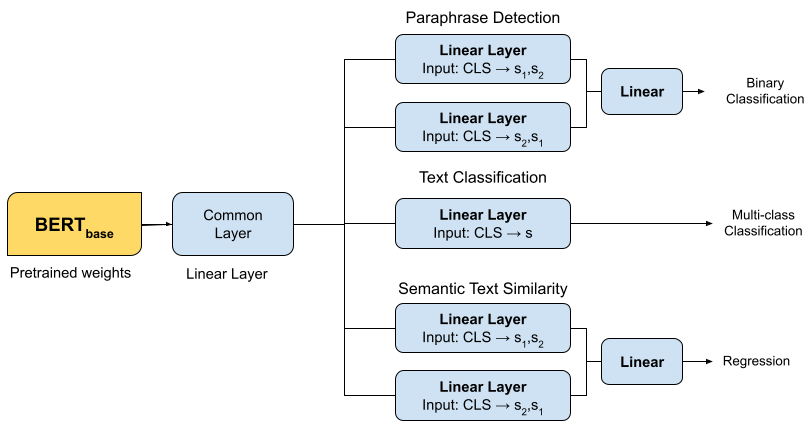
\includegraphics[width=10cm,keepaspectratio]{milestone/model.png}
    \label{fig:ModelArchitecture}
    \caption{Model architecture}
    % \caption{The figure provides an overview of the layers used in the current approach. A single dropout is applied }
\end{figure}

\begin{table}[htp]
\centering
\begin{tabular}{ |c|c|c|c|c| } 
 \hline
 \textbf{split} & \textbf{SST} & \textbf{CFIMDB} & \textbf{Quora} & \textbf{SemEval STS} \\
 \hline
 train & 8,544 & 1,701 & 141,506 & 6,041 \\
 \hline
 dev & 1,101 & 245 & 20,215 & 864 \\
 \hline
 test & 2,210 & 488 & 40,431 & 1,726\\  
 \hline
\end{tabular}
\caption{Dataset sizes for different splits \{\texttt{train}, \texttt{dev}, \texttt{test}\}}
\label{dataset-sizes}
\end{table}

\begin{table}[htp]
\centering
\begin{tabular}{|c|c|c|}
\hline
\textbf{Experiments} & \textbf{Model}                                 & \textbf{Training Method} \\ \hline
1                    & Vanilla                                        & Pretrain                 \\ \hline
2                    & Single Layers with logits                      & Finetune                 \\ \hline
3                    & Single Layers input concat pairs with 2 logits & Finetune                 \\ \hline
4                    & Additional Common layer                        & Finetune                 \\ \hline
5                    & Additional Common layer                        & Finetune                 \\ \hline
6                    & Additional Common layer with dropout           & Finetune                 \\ \hline
7                    & MT-DNN                                         & Finetune                 \\ \hline
\end{tabular}
\caption{Model and training method for different experiments}
\label{experiment-models}
\end{table}

\begin{table}[!htbp]
\centering
\begin{tabular}{|c|c|c|c|c|c|}
  \hline
  \textbf{Exp} &
  \textbf{Train Order} &
  \textbf{Epochs} &
  \textbf{lr} &
  \textbf{Batch Size} &
  \textbf{Dropout} \\
  \hline
  1 & SST only & 10 & 0.00001 & 32 & 0.3 \\
  \hline
  2 & QOP,SST,STS & 3 & 0.00001 & 32 & 0.5 \\
  \hline
  3 & SST,STS,SST,STS,QQP & 3 & 0.00001 & 32 & 0.5 \\
  \hline
  4 & STS,SST,QQP,SST,STS & 3 & 0.00001 & 32 & 0.5 \\
  \hline
  5 & STS,SST,QQP,SST,STS & 3 & 0.00001 & 16 & 0.5 \\
  \hline
  6 & STS,SST,SST,STS,QQP & 5 & 0.00001 & 32 & 0.1 \\
  \hline
  7 & Mixed & 5 & 0.00005 & 32 & 0.1 \\
  \hline
\end{tabular}
\caption{Changing hyperparamters for different experiments}
\label{experiment-hyperparameters}
\end{table}

% \begin{table}[!htbp]
% \centering
% \resizebox{\textwidth}{!}{%
% \begin{tabular}{|c|c|c|c|c|c|c|c|cccccc|c|}
% \hline
%   Experiments &
%   Model &
%   Training Method &
%   Train Order &
%   Epochs &
%   lr &
%   Batch Size &
%   dropout \\ \hline
   
% 1 &
%   Vanilla &
%   Pretrain &
%   SST only &
%   10 &
%   1.00E-05 &
%   32 &
%   0.3 &
%   \multicolumn{1}{c|}{0.393} &
%   \multicolumn{1}{c|}{0.388} &
%   \multicolumn{1}{c|}{0.008} &
%   \multicolumn{1}{c|}{-0.009} &
%   \multicolumn{1}{c|}{0.235} &
%   0.38 &
%   0.253 \\ \hline
% 2 &
%   Single Layers with logits &
%   Finetune &
%   QOP,SST,STS &
%   3 &
%   1.00E-05 &
%   32 &
%   0.5 &
%   \multicolumn{1}{c|}{0.491} &
%   \multicolumn{1}{c|}{0.327} &
%   \multicolumn{1}{c|}{0.883} &
%   \multicolumn{1}{c|}{0.866} &
%   \multicolumn{1}{c|}{0.824} &
%   0.764 &
%   0.652333333 \\ \hline
% \textbf{3} &
%   \textbf{Single Layers input concat pairs with 2 logits} &
%   \textbf{Finetune} &
%   \textbf{SST,STS,SST,STS,QQP} &
%   \textbf{3} &
%   \textbf{1.00E-05} &
%   \textbf{32} &
%   \textbf{0.5} &
%   \multicolumn{1}{c|}{\textbf{0.859}} &
%   \multicolumn{1}{c|}{\textbf{0.498}} &
%   \multicolumn{1}{c|}{\textbf{0.876}} &
%   \multicolumn{1}{c|}{\textbf{0.851}} &
%   \multicolumn{1}{c|}{\textbf{0.921}} &
%   \textbf{0.874} &
%   \textbf{0.741} \\ \hline
% 4 &
%   Additional Common layer &
%   Finetune &
%   STS,SST,QQP,SST,STS &
%   3 &
%   1.00E-05 &
%   32 &
%   0.5 &
%   \multicolumn{1}{c|}{0.846} &
%   \multicolumn{1}{c|}{0.499} &
%   \multicolumn{1}{c|}{0.948} &
%   \multicolumn{1}{c|}{0.875} &
%   \multicolumn{1}{c|}{0.896} &
%   0.822 &
%   0.732 \\ \hline
% 5 &
%   Additional Common layer &
%   Finetune &
%   STS,SST,QQP,SST,STS &
%   3 &
%   1.00E-05 &
%   16 &
%   0.5 &
%   \multicolumn{1}{c|}{0.876} &
%   \multicolumn{1}{c|}{0.483} &
%   \multicolumn{1}{c|}{0.95} &
%   \multicolumn{1}{c|}{0.878} &
%   \multicolumn{1}{c|}{0.891} &
%   0.810 &
%   0.723666667 \\ \hline
% 6 &
%   Additional Common layer with dropout &
%   Finetune &
%   STS,SST,SST,STS,QQP &
%   5 &
%   1.00E-05 &
%   32 &
%   0.1 &
%   \multicolumn{1}{c|}{0.964} &
%   \multicolumn{1}{c|}{0.454} &
%   \multicolumn{1}{c|}{0.968} &
%   \multicolumn{1}{c|}{0.864} &
%   \multicolumn{1}{c|}{0.935} &
%   0.794 &
%   0.704 \\ \hline
% 7 &
%   MT-DNN &
%   Finetune &
%   Mixed &
%   5 &
%   5.00E-05 &
%   32 &
%   0.1 &
%   \multicolumn{6}{c|}{To be Implemented} &
%   N/A \\ \hline
% \end{tabular}%
% }
% \caption{}
% \label{experiments-vanilla}
% \end{table}



\end{document}

